\documentclass[aspectratio=1610]{beamer}
\usepackage{hyperref}
\usepackage[T1]{fontenc}

% other packages
\usepackage{latexsym,amsmath,xcolor,multicol,booktabs,calligra}
\usepackage{graphicx,pstricks,listings,stackengine}
\usepackage{ragged2e}
\usepackage[backend=bibtex,sorting=none]{biblatex} % biblatex
\setbeamerfont{footnote}{size=\tiny}
% \addbibresource{ref.bib}

\usepackage{lipsum}

\author{Zhouxin Xue, Xuanhang Diao}
\title{Scheduling Beyond CPUs for HPC}
\subtitle{Fan Y, Lan Z, Rich P, et al. \\
\textit{HPDC 19} 
}

\institute{
    School of Biomedical Engineering, \\
    ShanghaiTech University \\
}
\date{14, April}
\usepackage{shanghaitech}

% defs
\def\cmd#1{\texttt{\color{red}\footnotesize $\backslash$#1}}
\def\env#1{\texttt{\color{blue}\footnotesize #1}}
\definecolor{deepblue}{rgb}{0,0,0.5}
\definecolor{deepred}{rgb}{0.6,0,0}
\definecolor{deepgreen}{rgb}{0,0.5,0}
\definecolor{halfgray}{gray}{0.55}

\lstset{
    basicstyle=\ttfamily\small,
    keywordstyle=\bfseries\color{deepblue},
    emphstyle=\ttfamily\color{deepred},    % Custom highlighting style
    stringstyle=\color{deepgreen},
    numbers=left,
    numberstyle=\small\color{halfgray},
    rulesepcolor=\color{red!20!green!20!blue!20},
    frame=shadowbox,
}

\begin{document}

\begin{frame}
    \titlepage
    \begin{figure}[htpb]
        \begin{center}
            
\includegraphics[keepaspectratio, scale=0.2]{pic/ShanghaiTech_Logo.png}
        \end{center}
    \end{figure}
\end{frame}

\section{Background Knowledge}

\begin{frame}{Pareto set}
    A \textbf{Pareto set} is a set of optimal solutions, where no objective can be improved without worsening another objective.
\end{frame}

\begin{frame}{Burst Buffer}
    A \textbf{Burst Buffer} is an intermediate storage layer positioned between compute nodes and parallel file systems (PFS) in high-performance computing (HPC) systems. 
    \begin{itemize}
        \item Absorb the bursty I/O data generated by data-intensive applications.
        \item Built from solid-state drives (SSDs).
        \item Can be either attached to compute nodes as local resources or configured as global resources shared by compute nodes.
    \end{itemize}
\end{frame}

\section{Background and Motivation}

\begin{frame}{Multi-Resource Scheduling}

    \begin{itemize}
        \item HPC systems are equipped with diverse global and local resources.
        \item HPC job scheduler plays a crucial role in efficient use of resources.
    \end{itemize}

    \begin{figure}[htpb]
        \begin{center}
            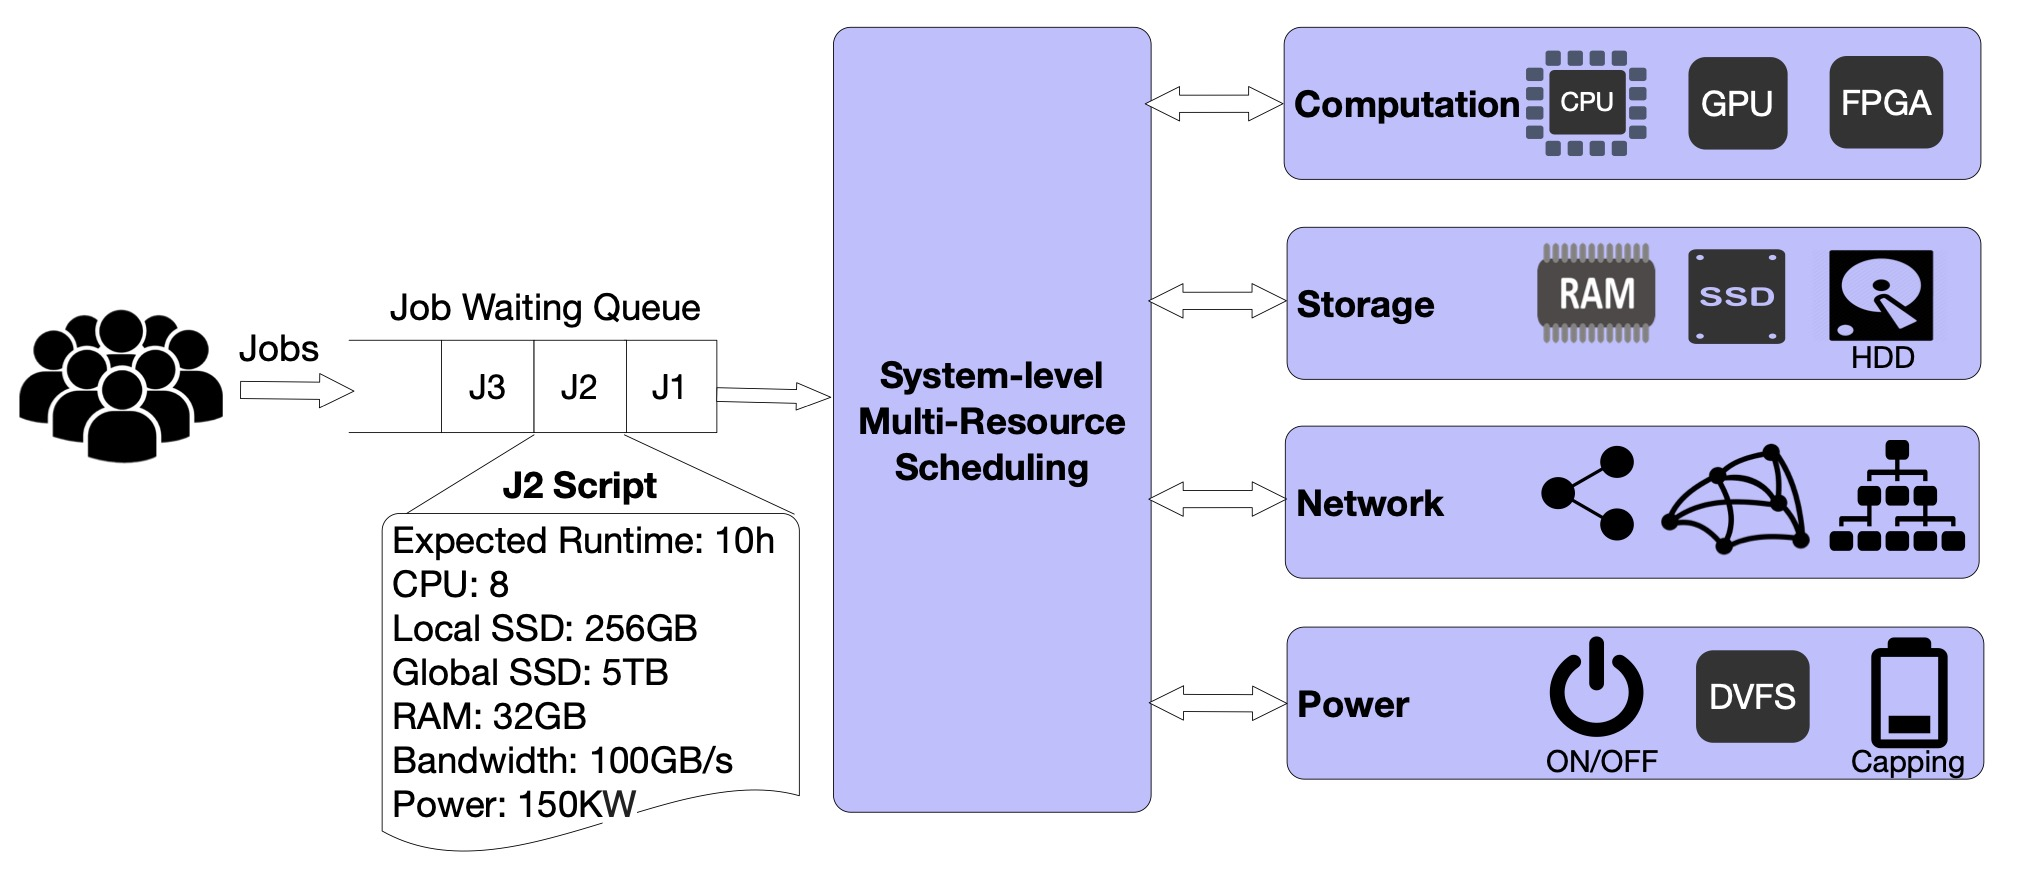
\includegraphics[keepaspectratio, scale=0.12]{pic/sched_with_multi_res.jpeg}
        \end{center}
        \caption{HPC job scheduling problem involves in multiple resources.}
        \label{fig:sched_with_multi_res}
    \end{figure}
   
\end{frame}

\begin{frame}{Limitations of Existing Scheduling Methods}
    
    Existing methods often overlook alternative solutions or optimal resource combinations, leading to under-utilization of resources or poor application performance.
    
    \begin{itemize}
        \item Naive method
        \item Constrained method
        \item Weighted method
        \item Bin packing method
    \end{itemize}
    
\end{frame}

\begin{frame}{Goal}

    The Motivation of the this paper is to improve overall resource utilization and reduce job wait time in HPC systems.

    \begin{itemize}
        \item providing rapid scheduling decisions
        \item minimizing the impact on site policies
        \item ensuring extensibility to accommodate emerging resources
    \end{itemize}
   
\end{frame}

\section{Methodology of BBSched}

\begin{frame}{Window-based Scheduling}
    The idea of window-based scheduling as shown is that the first $w$ jobs in the job waiting queue get copied into the window.   \\

    This allows our BBsched to consider the site policies and keep the order of the base scheduler as similar as possible. \\
    \begin{figure}[htpb]
        \centering
        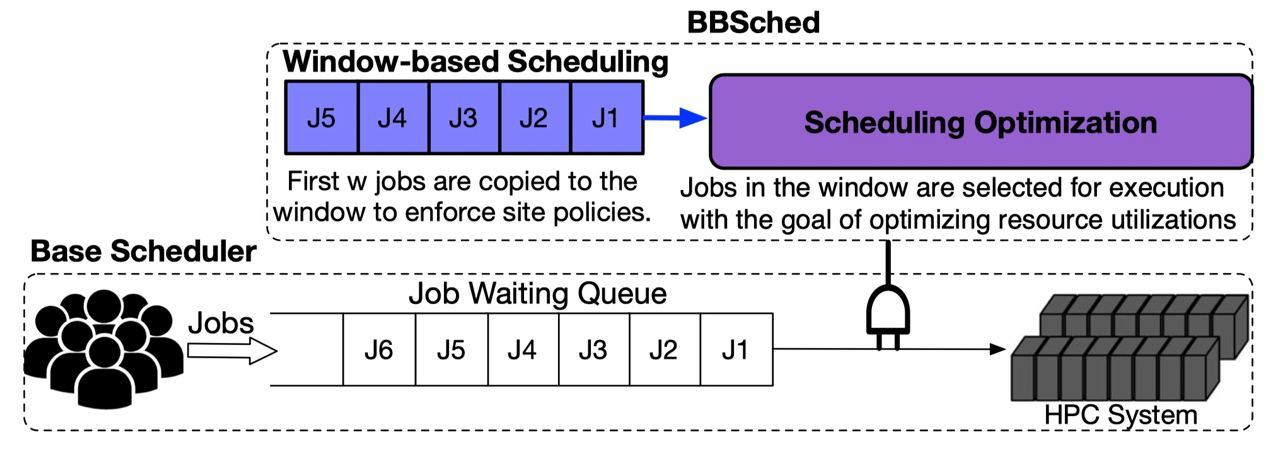
\includegraphics[keepaspectratio, scale=0.2]{pic/BBSched.jpg}
        \caption{The overview of BBsched.}
        \label{fig:BBsched}
     \end{figure}
\end{frame}

\begin{frame}{MOO Solver}

    Suppose a system has $N$ nodes and burst buffers of total $B$ GB. 
    The amounts of nodes and burst buffers being used are $N_{used}$ and $B_{used}$ respectively.
    Suppose $J = \{J_1 , . . . , J_w \} $is a set of $w$ jobs in the scheduling window. 
    Job $J_i$ requiring $n_i$ nodes and $b_i $GB of burst buffers. \\
    \vspace{10pt}
    The scheduling problem can be transformed into the following MOO: 
    to determine a finite set of Pareto solutions $X$; 
    each Pareto solution $x \in X$ is represented by a binary vector $x = [x_1 , . . . ,x_w ]$, 
    such that $x_i = 1$ if $J_i$ is selected to execute and $x_i = 0$ otherwise. \\
    \vspace{10pt}
    Pareto solution optimizes the following two objectives: \\
    (1) maximize node utilization:  $f_{1}(\boldsymbol{x})=\sum_{i=1}^{w} n_{i} \times x_{w}$ \\
    (2) maximize burst buffer utilization:  $f_{2}(\boldsymbol{x})=\sum_{i=1}^{w} b_{i} \times x_{i}$ \\  
    Formally, the problem can be formulated as:
    $$
    \begin{array}{ll}
    \max & \left(f_{1}(\boldsymbol{x}), f_{2}(\boldsymbol{x})\right) \\
    \text { s.t. } & \sum_{i=1}^{w} n_{i} \times x_{i} \leq N-N_{\text {used }}, \quad x_{i} \in\{0,1\} \\
    & \sum_{i=1}^{w} b_{i} \times x_{i} \leq B-B_{\text {used }}, \quad x_{i} \in\{0,1\}
    \end{array}
    $$

\end{frame}

\begin{frame}{MOO Solver}
    Because this MOO problem is NP-hard, this paper uses a genetic algorithm to approximate the Pareto set (optimal solutions). \\
    \begin{figure}
        \begin{center}
            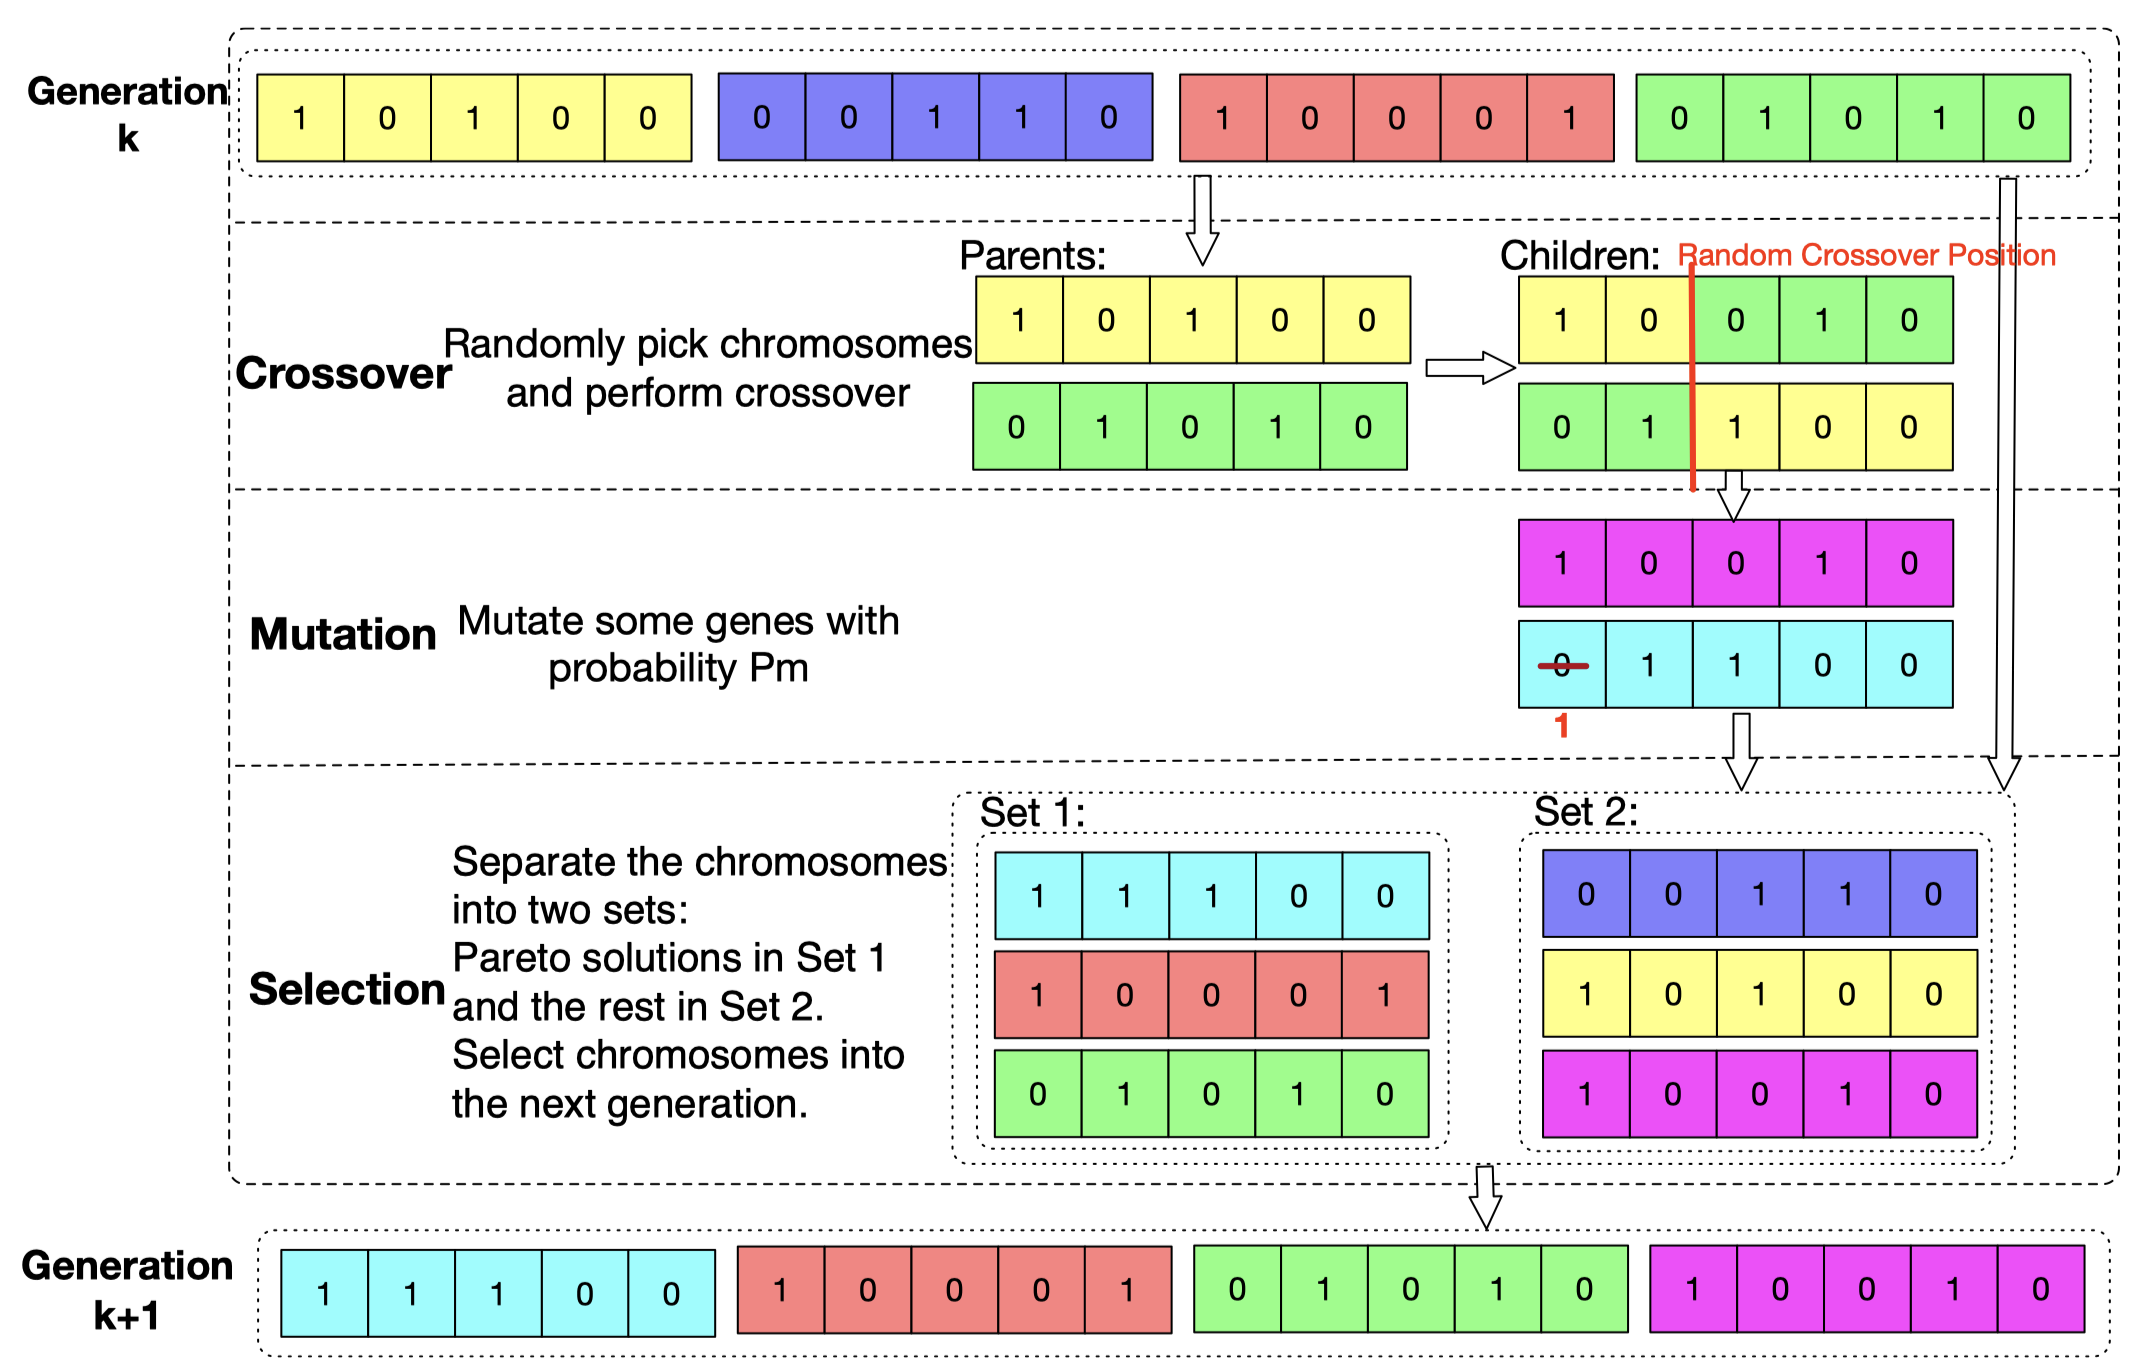
\includegraphics[keepaspectratio, scale=0.18]{pic/genetic.png}
            \caption{MOO solver maintains a population of candidate solutions (4 chromosomes). 
            A chromosome consists of 5 genes, where each gene represents the selection of the job at a specific location in the window and encodes as a binary number: 1 (selected) or 0 (not selected).}
            \label{fig:Genetic_Algorithm}
        \end{center}
    \end{figure}
\end{frame}

\begin{frame}{Decision making}
    The output of the solver is a Pareto set, and a decision maker needs to select one preferred solution. \\
    \vspace{10pt}
    Different HPC facilities may have different site policies and scheduling priorities. \\
    \vspace{10pt}
    System managers may use a site-specific metric for selecting a preferred solution out of the Pareto set. 
\end{frame}

\section{Evaluation}

\begin{frame}{Workloads}
    Simulation using real workload traces collected from production systems.
    \begin{figure}
        \centering
        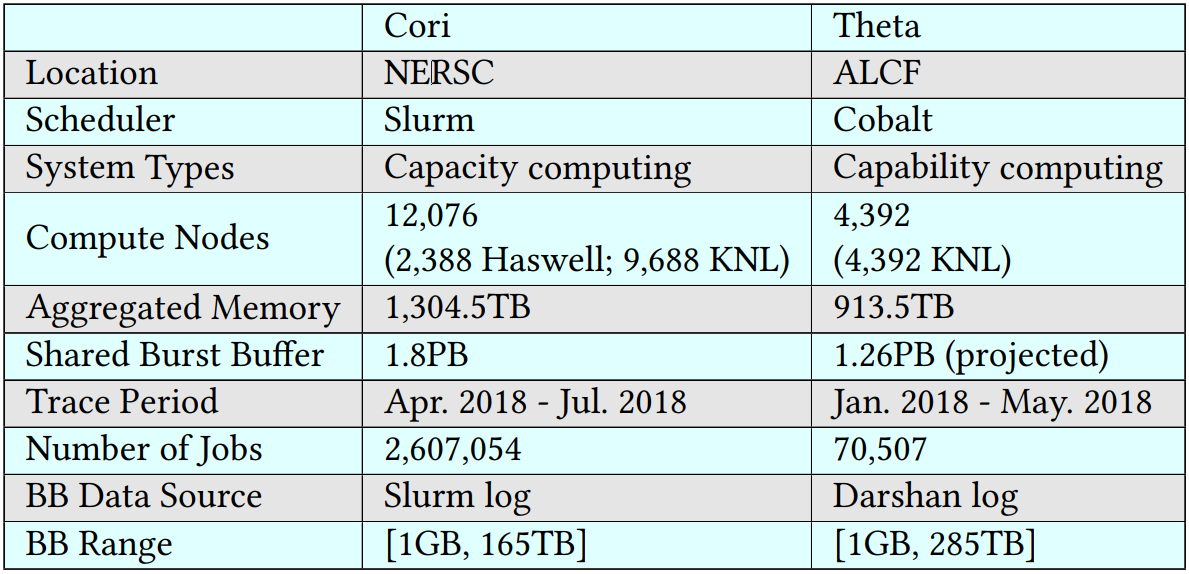
\includegraphics[scale=0.4]{pic/workload.png}
        \caption{Overview of Cori and Theta workloads}
        \label{fig:workload}
    \end{figure}
    \begin{itemize}
    \item Theta is currently not deployed with any shared burst buffer (set the more than 1GB of transferred data as the corresponding job’s burst buffer request)
\end{itemize}
\end{frame}

\begin{frame}{Workload Settings}
\begin{table}[]
\begin{tabular}{|c|c|c|}
\hline
Workload & percentage of jobs requesting BB & assigned burst buffer request \\ \hline
S1       & $50\%$                           & $\geq 5$TB                    \\ \hline
S2       & $75\%$                           & $\geq 20$TB                   \\ \hline
S3       & $50\%$                           & $\geq 5$TB                    \\ \hline
S4       & $75\%$                           & $\geq 20$TB                   \\ \hline
\end{tabular}
\end{table}
\begin{itemize}
    \item One issue with both traces is that original burst buffers are not heavily used, and expecting significant increases in requests for burst buffers.
    \item the assigned burst buffer request is randomly selected from the original burst buffer requests.
    
\end{itemize}
\end{frame}

\begin{frame}{Workload Settings}
\begin{figure}
    \centering
    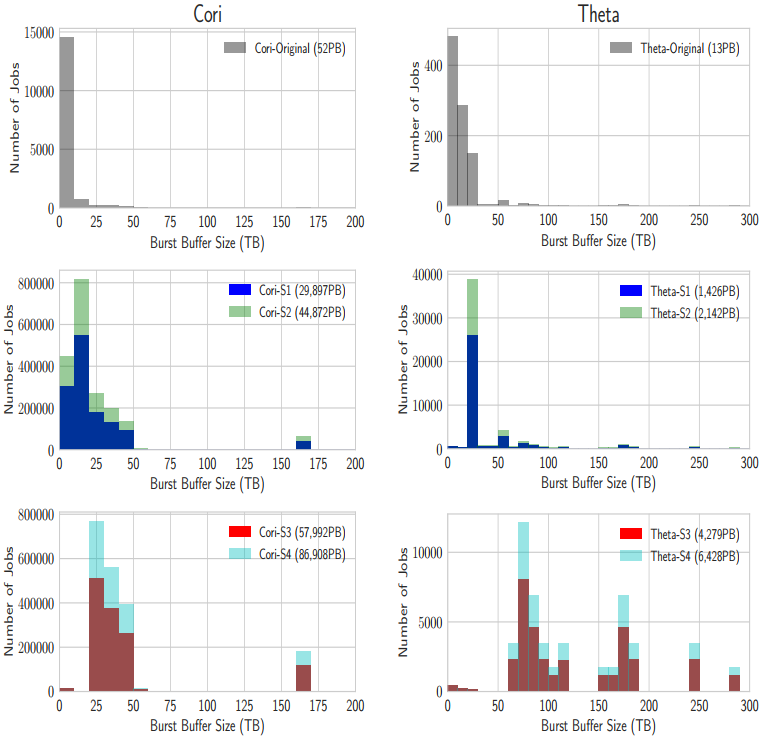
\includegraphics[scale=0.40]{pic/workload_reset.png}
    \caption{S3 and S4 workloads have larger burst buffer requests than S1 and S2. S1 and S2 have similar distributions, but more jobs in S2 request burst
    buffers}
    \label{fig:my_label}
\end{figure}    
\end{frame}

\begin{frame}{Metrics}
The first two metrics are system-level performance metrics, whereas the last two are user-level performance metrics
\begin{enumerate}
    \item Node usage: running time/allocate time
    \item Burst buffer usage: using time/allocate time
    \item Job wait time: interval between job submission to job start time
    \item Job slowdown: (job runtime + wait time)/actual runtime
\end{enumerate}
\end{frame}

\begin{frame}{Methods}
    Eight multi-resource scheduling methods:
\begin{enumerate}
    \item Baseline
    \item Weighted: weights of node 50\% - weight of BB 50\%
    \item Weighted\_CPU: weights of node 80\% - weight of BB 20\%
    \item Weighted\_BB:  weights of node 20\% - weight of BB 80\%
    \item Constrained\_CPU: maximize node utilization
    \item Constrained\_BB:maximize burst buffer utilization 
    \item Bin\_Packing:compute a dot product between the vector of available and requested resources for jobs, then allocate jobs with highest alignment score recursively
    \item BBSched: window size to 20, the number of generation to 500, the population size to 20, and the mutation probability to 0.05\%
\end{enumerate}
\end{frame}

\section{Result}

\begin{frame}{Overview of Result}
    \begin{figure}
        \centering
        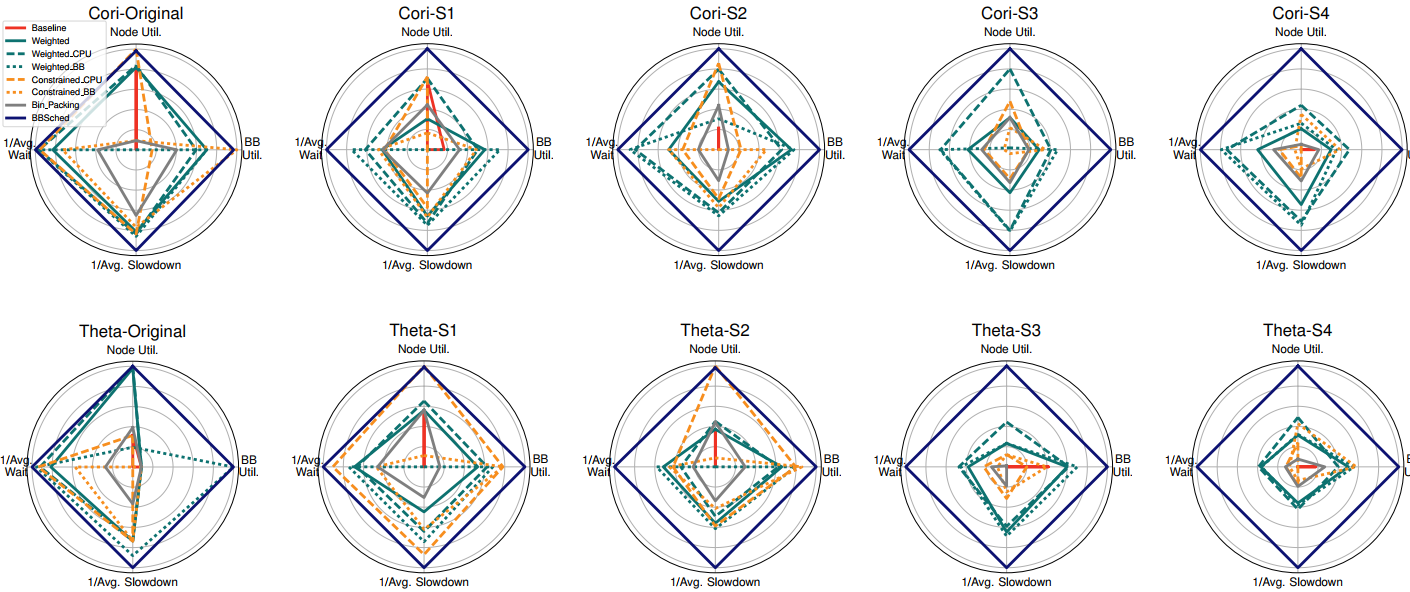
\includegraphics[scale=0.247]{pic/overall_performence.png}
        \caption{Kiviat graphs: Cori traces (top) and Theta traces (bottom).The
            larger the area is, the better the overall performance is.}
        \label{fig:my_label}
    \end{figure}
\end{frame}

\begin{frame}{Nodes and Buffer Usage}
    \begin{figure} \centering
        \subfigure { \label{fig:a}
        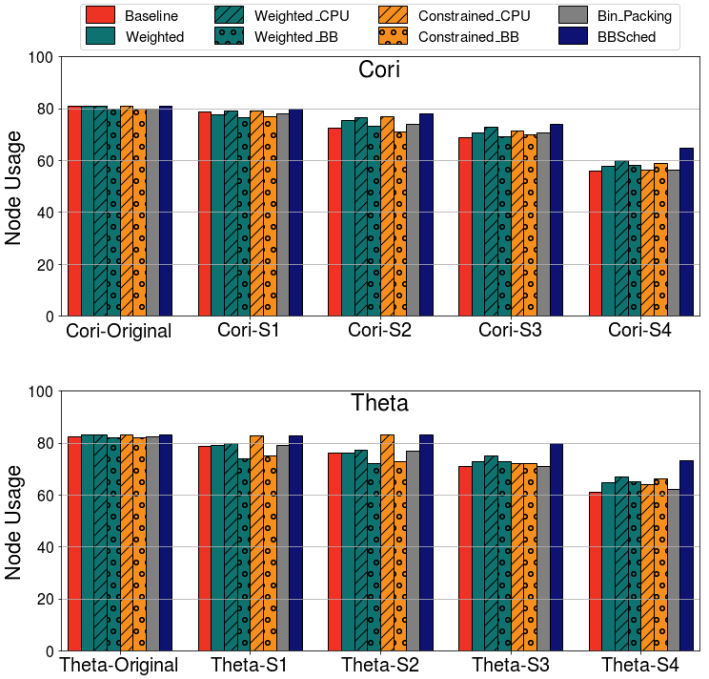
\includegraphics[width=0.47\columnwidth]{pic/node_usage.png}
        }
        \subfigure{ \label{fig:b}
        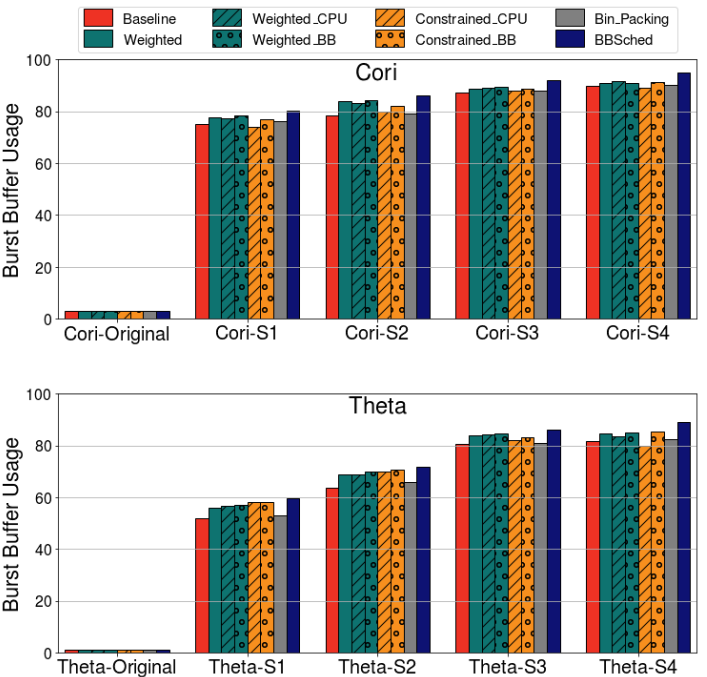
\includegraphics[width=0.47\columnwidth]{pic/buffer_usage.png}
        }
    \label{fig}
    \end{figure}
    \begin{itemize}
        \item  Node usage and BB usage are almost negatively correlated.
        \item Where's the sweet point?
    \end{itemize}
\end{frame}

\begin{frame}{Wait Time}
    \begin{figure} \centering
        \subfigure { \label{fig:a}
        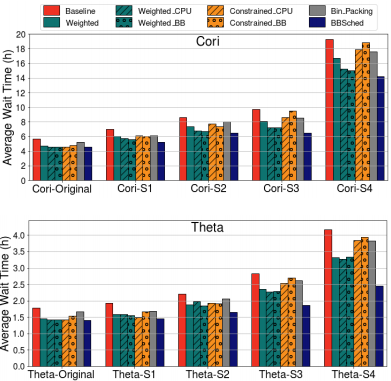
\includegraphics[width=0.47\columnwidth]{pic/wait_time.png}
        }
        \subfigure{ \label{fig:b}
        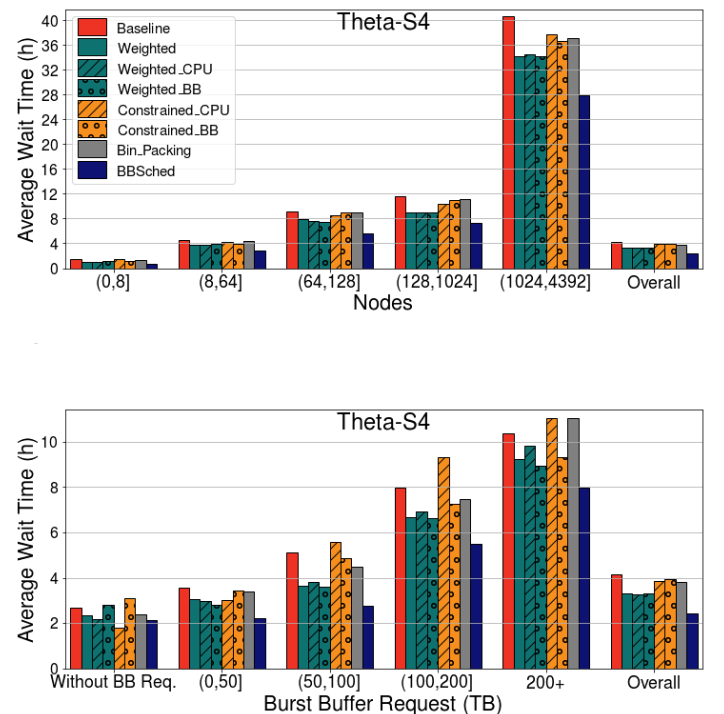
\includegraphics[width=0.47\columnwidth]{pic/wait_analy.png}
        }
    \label{fig}
    \end{figure}
    \begin{itemize}
        \item BBSched achieves the most significant reductions on average job
            wait time, the most significant gain comes from small jobs.
        \item all optimization methods reduce average wait time of long jobs, but increase the average wait time of short jobs. 
    \end{itemize}
\end{frame}

\begin{frame}{Sensitivity Analysis}
\begin{figure}
    \centering
    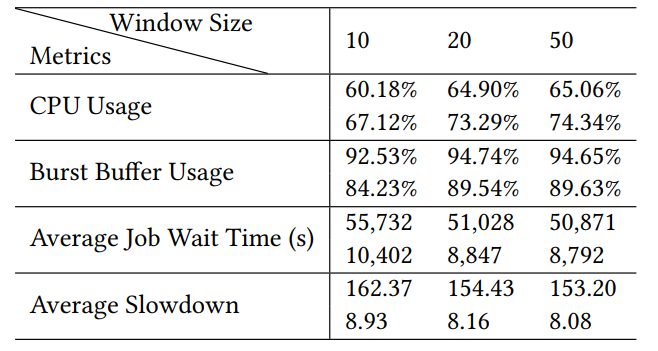
\includegraphics[scale=0.5]{pic/sensititity.png}
    \caption{ BBSched performance under different window sizes. There are two numbers per cell: the top is for Cori-S4 and the bottom is for Theta-S4}
\end{figure}
Window sizes between 10 to 30 have no significant effect. But a range of 10 to 20 is best.
\end{frame}


\section{Incorporate More Resources}

\begin{frame}{Incorporate Additional Resources}
 Present a case study to illustrate that BBSched can be easily extended to incorporate additional schedulable resources. Add two additional objectives
 \begin{itemize}
     \item  maximize local SSD utilization
     \item  minimize wasted local SSD
 \end{itemize}
For hardware configuration, assume 50\% of nodes in the system are equipped with 128 GB local SSDs, the rest of the nodes are equipped with 256 GB local SSDs.

Generate three workloads (S5-S7) based on Cori-S2 and Theta-S2 by
creating job’s local SSD requests

\begin{table}[]
\begin{tabular}{|c|c|c|}
\hline
Workload & 0-128G SSD request & 129-256G SSD request \\ \hline
S5       & $80\%$             & $20\%$               \\ \hline
S6       & $50\%$             & $50\%$               \\ \hline
S7       & $20\%$             & $80\%$               \\ \hline
\end{tabular}
\end{table}
 Weighted method aims to maximize the equally weighted sum of node, burst buffer, local SSD utilization, and negative percentage of wasted SSD. Constrained\_SSD method aims to maximize local SSD utilization under
the constraints of the other resources.
\end{frame}

\begin{frame}{More Complex Optimization Problems}
    \begin{figure}
        \centering
        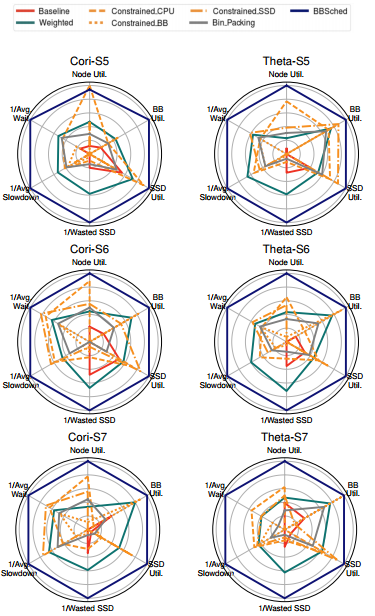
\includegraphics[scale=0.3]{pic/more_concern.png}
        \caption{BBSched achieves the best overall performance on all workloads}
    \end{figure}
\end{frame}

\section{Conclusion}

\begin{frame}{Conclusion}
    \begin{itemize}
        \item Multi-resource scheduling problem can be formulated into a MOO problem and is rapidly solved by a multi-objective genetic algorithm.
        \item  The extensive trace-based simulations demonstrate BBSched outperforms the existing methods in terms of both system-level and user-level metrics(41\% over naive method, 33\% over bin packing method, 35\% over constrained methods, and 20\% over weighted methods). 
        \item  Can be extended to incorporate other resources.
        \item Needs test on real systems.
    \end{itemize}
\end{frame}
\end{document}